\documentclass[aspectratio=169,11pt]{beamer}
\usetheme{default}
\usepackage{fontspec}
\usepackage{amsmath,amssymb,mathtools}
\usepackage{booktabs}
\usepackage{graphicx}
\usepackage[most]{tcolorbox}
\usepackage{microtype}

% ---------------- typography ----------------
\usefonttheme{serif}
\setmainfont{Charter}[Numbers=OldStyle]
\setsansfont{Avenir Next}
\renewcommand{\arraystretch}{1.15}

% ---------------- palette ----------------
\definecolor{ink}{HTML}{15293C}
\definecolor{accent}{HTML}{BF5B1D}
\definecolor{muted}{HTML}{6E7D8A}
\definecolor{wash}{HTML}{F5F2ED}
\definecolor{rule}{HTML}{D8D2C8}

\setbeamercolor{normal text}{fg=ink}
\setbeamercolor{structure}{fg=accent}
\setbeamercolor{itemize item}{fg=accent}
\setbeamercolor{itemize subitem}{fg=muted}
\setbeamercolor{enumerate item}{fg=accent}
\setbeamerfont{frametitle}{family=\sffamily,series=\bfseries,size=\large}
\setbeamerfont{title}{family=\sffamily,series=\bfseries,size=\LARGE}
\setbeamerfont{author}{size=\scriptsize}
\setbeamerfont{institute}{size=\scriptsize}
\setbeamerfont{date}{size=\scriptsize}
\setbeamertemplate{navigation symbols}{}
\setbeamersize{text margin left=1.7em,text margin right=1.7em}
\setbeamertemplate{itemize item}{\small\raisebox{0.12em}{\rule{0.42em}{0.42em}}}
\setbeamertemplate{itemize subitem}{\scriptsize\raisebox{0.12em}{\rule{0.3em}{0.3em}}}

% frame title: left aligned, short accent rule beneath. No coloured bar.
\setbeamertemplate{frametitle}{%
  \vspace{1.0em}\hspace{0.2em}%
  \begin{minipage}{0.95\textwidth}
  {\usebeamerfont{frametitle}\color{ink}\insertframetitle\par}%
  \vspace{0.25em}{\color{accent}\rule{2.0em}{1.4pt}}%
  \end{minipage}\par\vspace{0.3em}%
}

% footline: a hairline and a page number. Nothing else.
\setbeamertemplate{footline}{%
  \hspace{1.6em}{\color{rule}\rule{\dimexpr\paperwidth-3.2em\relax}{0.4pt}}\par
  \vspace{0.25em}\hspace{1.6em}%
  {\sffamily\scriptsize\color{muted}Volatility as a quadratic variation\hfill
   \insertframenumber\hspace{1.6em}}\par\vspace{0.5em}%
}

% ---------------- callouts: left bar, no box frame ----------------
\newtcolorbox{callout}[1][]{enhanced,breakable,colback=wash,frame hidden,sharp corners,
  borderline west={2.2pt}{0pt}{accent},left=9pt,right=7pt,top=5pt,bottom=5pt,#1}
\newtcolorbox{inknote}[1][]{enhanced,breakable,colback=wash,frame hidden,sharp corners,
  borderline west={2.2pt}{0pt}{ink},left=9pt,right=7pt,top=5pt,bottom=5pt,#1}

\newcommand{\lead}[1]{{\sffamily\bfseries\color{accent}#1}}
\newcommand{\dd}{\mathrm{d}}
\newcommand{\half}{\tfrac{1}{2}}
\newcommand{\si}{\sigma_{\mathrm{imp}}}
\newcommand{\sr}{\sigma_{\mathrm{real}}}

% section divider
\newcommand{\divider}[3]{%
{\setbeamertemplate{footline}{}
\begin{frame}
\vfill
{\sffamily\scriptsize\color{accent}Stage #1}\par\vspace{0.3em}
{\sffamily\bfseries\Huge\color{ink}#2}\par\vspace{0.6em}
{\color{rule}\rule{0.42\textwidth}{0.6pt}}\par\vspace{0.5em}
{\color{muted}#3}
\vfill
\end{frame}}}

\begin{document}

% ---------------- title ----------------
{\setbeamertemplate{footline}{}
\begin{frame}
\vspace{1.4em}
{\sffamily\scriptsize\color{accent}MAC F244 \ \ \textbullet\ \ Project Component}\par
\vspace{1.1em}
{\sffamily\bfseries\Huge\color{ink}Volatility as a quadratic variation}\par
\vspace{0.45em}
{\Large\color{muted}Measuring it, forecasting it, and pricing it on the NIFTY 50}\par
\vspace{0.9em}
{\color{accent}\rule{3.2em}{1.6pt}}\par
\vspace{1.0em}
{\sffamily\scriptsize\color{ink}
Jaivin Bengani \textcolor{muted}{2024ADPS0850G}\ \ \textbullet\ \
Purunjay Karwa \textcolor{muted}{2024ADPS0857G}\ \ \textbullet\ \
Soham Agrawal \textcolor{muted}{2024ADPS0829G}\par
\vspace{0.35em}
Vrishank Bimlesh Rao \textcolor{muted}{2024ADPS0871G}\ \ \textbullet\ \
Bhagyesh \textcolor{muted}{2024ADPS0863G}}\par
\vspace{1.0em}
{\sffamily\scriptsize\color{muted}Stochastic Calculus and Applications to Finance\ \ \textbullet\ \
Prof.\ Mayank Goel\ \ \textbullet\ \ BITS Pilani, K.\ K.\ Birla Goa Campus}
\end{frame}}

% ---------------- problem ----------------
\begin{frame}{One input you cannot observe}
Black--Scholes takes five inputs.
\vspace{0.5em}

\hspace{1.2em}\begin{minipage}{0.86\textwidth}
{\sffamily\color{muted}Spot \ \textbullet\ \ Strike \ \textbullet\ \ Time to maturity \ \textbullet\ \
Interest rate}\par
\vspace{0.25em}
{\color{muted}All four are on a screen.}\par
\vspace{0.7em}
{\sffamily\bfseries\color{accent}Volatility $\sigma$}\par
\vspace{0.1em}
A property of the \emph{future}. Nobody publishes it.
\end{minipage}
\vspace{0.9em}

\begin{callout}
The usual workaround is to choose the $\sigma$ that reproduces the price you already see and
call it implied volatility. That assumes the answer in order to obtain it.
\end{callout}
\vspace{0.4em}
The derivation done in class treats $\sigma$ as given.
\lead{This project removes that asymmetry using nothing beyond the course.}
\end{frame}

% ---------------- identity ----------------
\begin{frame}{The identity everything rests on}
Apply It\^o's lemma to $f(S)=\log S$ under $\dd S_t=\mu_tS_t\dd t+\sigma_tS_t\dd W_t$, then take
the quadratic variation. The drift contributes nothing at first order and $(\dd W)^2=\dd t$:
\vspace{-0.2em}
\[{\color{ink}[\log S]_T\;=\;\int_0^T\sigma_t^2\,\dd t}\]
\vspace{-1.0em}
\begin{columns}[T]
\begin{column}{0.47\textwidth}
\lead{Left side}\par Computable from closing prices. Sum the squared log differences.
\end{column}
\begin{column}{0.47\textwidth}
\lead{Right side}\par The quantity nobody can see.
\end{column}
\end{columns}
\vspace{0.8em}
The sample version is realised variance, $RV_n=\sum(\Delta\log S)^2$.\par
\vspace{0.2em}
\lead{Volatility stops being a fitted parameter and becomes a measurement.}
\end{frame}

% ---------------- roadmap ----------------
\begin{frame}{Three stages, each a prerequisite for the next}
\begin{columns}[T]
\begin{column}{0.30\textwidth}
{\sffamily\scriptsize\color{accent}01}\par
{\sffamily\bfseries\color{ink}Verify}\par\vspace{0.3em}
\small Test the estimator where $\sigma(t)$ was chosen by us, so the true answer is known
independently.
\end{column}
\begin{column}{0.30\textwidth}
{\sffamily\scriptsize\color{accent}02}\par
{\sffamily\bfseries\color{ink}Measure}\par\vspace{0.3em}
\small Apply it to eleven years of NIFTY 50 and establish precisely which assumptions of
constant-$\sigma$ GBM fail.
\end{column}
\begin{column}{0.30\textwidth}
{\sffamily\scriptsize\color{accent}03}\par
{\sffamily\bfseries\color{ink}Price}\par\vspace{0.3em}
\small Compare measurement against the market's quote, then derive and independently confirm
what the gap is worth.
\end{column}
\end{columns}
\vspace{1.1em}
\begin{inknote}
\small\lead{Data.}\ NIFTY 50 and India VIX daily closes, 2 January 2015 to 12 November 2026.
\textbf{2,903 trading days}, no missing values. Retrieved with \texttt{yfinance} and validated
on ingest for ordering, duplicates, positivity and calendar gaps.
\end{inknote}
\end{frame}

\divider{01}{Verify}{Check the ruler before measuring anything with it.}

% ---------------- verification ----------------
\begin{frame}{The estimator does what the theory says}
Simulate with $\sigma(t)=0.15+0.10\sin(2\pi t)$, for which $\int_0^1\sigma^2\dd t=0.027500$ by
hand. Use the \emph{exact} log-solution of GBM, so no discretisation error contaminates the test.
\vspace{0.3em}
\begin{columns}[T]
\begin{column}{0.54\textwidth}
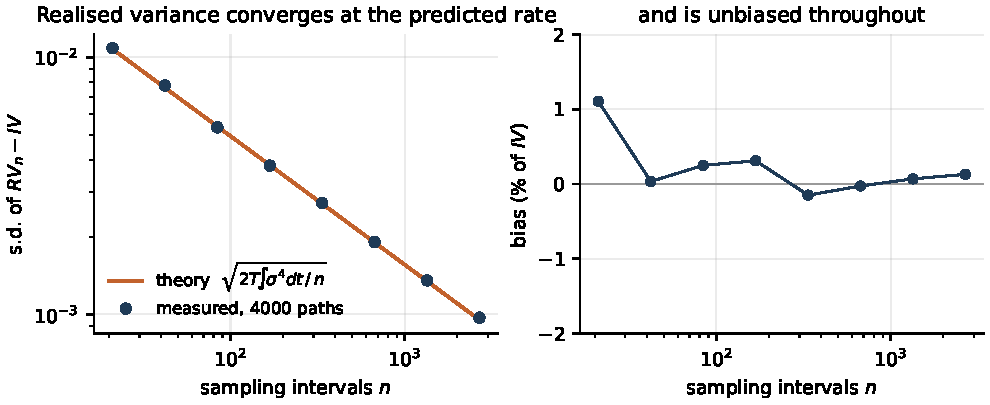
\includegraphics[width=\linewidth]{figures/rv_convergence.pdf}
\end{column}
\begin{column}{0.44\textwidth}
\small
\begin{tabular}{@{}ll@{}}
\toprule
Predicted slope & $-1/2$\\
\textbf{Measured} & $\mathbf{-0.4986}$\\
\addlinespace
\multicolumn{2}{@{}l@{}}{\footnotesize Dispersion vs $\sqrt{(2T/n)\int\sigma_t^4\dd t}$}\\
\textbf{ratio} & $\mathbf{0.991}$ to $\mathbf{1.021}$\\
across & a $128\times$ range of $n$\\
\bottomrule
\end{tabular}
\vspace{0.7em}

{\footnotesize\color{muted}The constant 2 comes from
$\mathrm{Var}\big((\Delta W)^2\big)=2(\Delta t)^2$, since $(\Delta W)^2/\Delta t\sim\chi^2_1$.}
\end{column}
\end{columns}
\vspace{0.4em}
\lead{We test the constant, not merely the rate.}
\end{frame}

\divider{02}{Measure}{Eleven years of NIFTY 50, and exactly how the model fails.}

% ---------------- measurement ----------------
\begin{frame}{Three assumptions fail, in three specific ways}
Realised volatility averages $14.17\%$ and spans $5.37\%$ to $88.45\%$. No constant
approximates that. The \emph{manner} of failure is what matters.
\vspace{0.5em}
\begin{columns}[T]
\begin{column}{0.46\textwidth}
\small
\begin{tabular}{@{}lr@{}}
\toprule
Ljung--Box $Q(10)$, squared returns & $\mathbf{1752.1}$\\
Ljung--Box $Q(10)$, returns & $59.3$\\
$\chi^2_{10}$ critical value, $1\%$ & $23.2$\\
\addlinespace
Leverage, $\mathrm{corr}(r_t,\Delta\hat\sigma_t)$ & $\mathbf{-0.200}$\\
Excess kurtosis & $19.3$\\
\bottomrule
\end{tabular}
\end{column}
\begin{column}{0.50\textwidth}
\small
\lead{Clustering.}\ The \emph{size} of tomorrow's move is strongly predictable. GBM implies
zero autocorrelation at every lag.
\vspace{0.5em}

\lead{Asymmetry.}\ Volatility rises on down moves. GBM is symmetric in $W$ and cannot produce
this, which is why a skew exists.
\end{column}
\end{columns}
\vspace{0.7em}
{\color{muted}Hold on to this. It is what makes the result three slides from now surprising.}
\end{frame}

\divider{03}{Price}{What the measurement is worth once the market disagrees with it.}

% ---------------- MZ ----------------
\begin{frame}{The market's own forecast is biased}
India VIX is a model-free 30-day implied volatility, built from traded NIFTY option prices by
the variance-swap construction. Regress what happened on what was predicted, over
\textbf{138 non-overlapping} cycles:
\vspace{-0.1em}
\[\sr=a+b\,\si+\varepsilon,\qquad
  \hat a=0.0310\,(0.0163),\quad \hat b=0.6637\,(0.0909),\quad R^2=0.282\]
\vspace{-0.9em}

Unbiasedness requires $a=0$, $b=1$. The slope is rejected at $t_{b=1}=\mathbf{-3.70}$.
\vspace{0.6em}
\begin{callout}
A one-point rise in India VIX is followed on average by only \textbf{two-thirds} of a point of
extra realised volatility. The forecast is informative but \textbf{overreacts}. Mean gap
$\mathbf{+2.50}$ volatility points, $t=4.04$, positive in $\mathbf{76.8\%}$ of months. This is
the \textbf{variance risk premium}.
\end{callout}
\vspace{0.3em}
{\footnotesize\color{muted}Windows are non-overlapping so the standard errors are not inflated
by induced serial correlation.}
\end{frame}

% ---------------- P&L identity ----------------
\begin{frame}{What It\^o says that gap is worth}
Impose self-financing, apply It\^o, substitute the Black--Scholes PDE. The $\dd W$ terms cancel
exactly, because $\Delta=V_S$:
\vspace{-0.1em}
\[{\color{ink}\Pi_T=\half\int_0^T e^{r(T-t)}\,S_t^2\,\Gamma_t\,\big(\si^2-\sigma_t^2\big)\,\dd t}\]
\vspace{-0.9em}
\begin{itemize}
  \item The whole P\&L is an integral of \textbf{dollar gamma} against the
        \textbf{variance gap}.
  \item A \emph{pathwise} identity. Once the path is fixed nothing random remains.
  \item It needs only that $S$ be a continuous semimartingale with quadratic variation
        $\int\sigma_t^2\dd t$, \lead{the object Stage 01 verified.}
\end{itemize}
\vspace{0.4em}
It does \textbf{not} need normality, independence, or constant $\sigma$.
\end{frame}

% ---------------- hero number ----------------
{\setbeamertemplate{footline}{}
\begin{frame}
\vfill
\centering
{\sffamily\footnotesize\color{muted}It\^o's prediction against realised P\&L, 138 months}\par
\vspace{0.4em}
{\sffamily\bfseries\fontsize{76}{76}\selectfont\color{accent}0.949}\par
\vspace{0.7em}
{\color{ink}\large Two independent procedures. One shared price path.}\par
\vspace{0.3em}
{\color{muted}Predicted $+39.21$ points per cycle against an actual $+36.06$.}
\vfill
\end{frame}}

% ---------------- the check ----------------
\begin{frame}{Why that number means something}
\begin{columns}[T]
\begin{column}{0.44\textwidth}
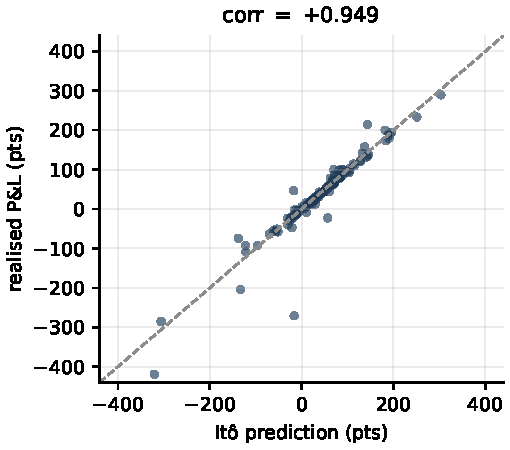
\includegraphics[height=0.45\textheight]{figures/ito_vs_actual.pdf}
\end{column}
\begin{column}{0.52\textwidth}
\footnotesize
\lead{Route A}\ \ Evaluate the It\^o integral by quadrature along each realised NIFTY path.
\vspace{0.45em}

\lead{Route B}\ \ Simulate the hedge as pure accounting: borrow, rebalance daily, settle at
expiry.
\vspace{0.6em}

\begin{tabular}{@{}lr@{}}
\toprule
Predicted & $+39.21$ pts\\
Actual & $+36.06$ pts\\
\textbf{Correlation} & $\mathbf{+0.9493}$\\
\bottomrule
\end{tabular}
\end{column}
\end{columns}
\vspace{0.3em}
\begin{callout}
\footnotesize The P\&L is never computed \emph{from} the formula. Had it been, agreement would
be guaranteed and would mean nothing. The two procedures share only the price path.
\end{callout}
\end{frame}

% ---------------- backtest ----------------
\begin{frame}{The premium is real and economically sized}
\begin{columns}[T]
\begin{column}{0.54\textwidth}
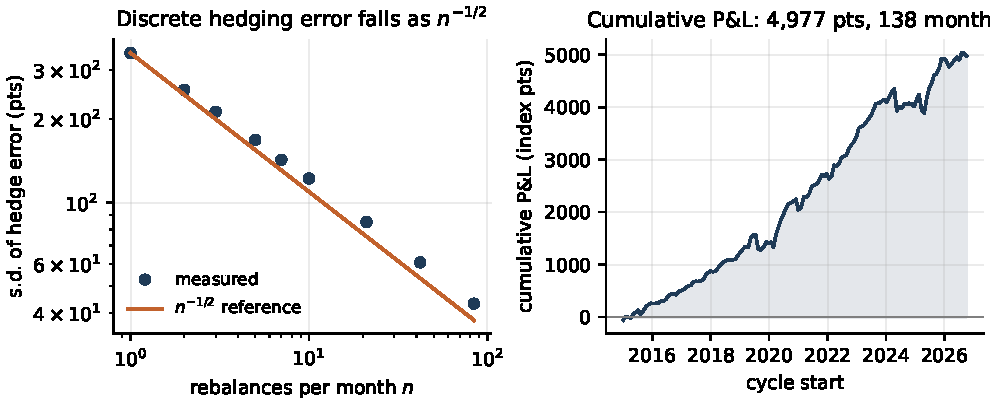
\includegraphics[width=\linewidth]{figures/hedge.pdf}
\end{column}
\begin{column}{0.44\textwidth}
\small
\begin{tabular}{@{}lr@{}}
\toprule
Mean P\&L per cycle & $+36.06$ pts\\
Share of premium & $+11.31\%$\\
Win rate & $74.6\%$\\
$t$-statistic & $4.80$\\
$p$-value & $4.1\times10^{-6}$\\
Cumulative, 138 months & $+4{,}977$ pts\\
\bottomrule
\end{tabular}
\vspace{0.8em}

{\footnotesize\color{muted}Short an at-the-money call, delta-hedged daily, rolled monthly over
eleven years.}
\end{column}
\end{columns}
\end{frame}

% ---------------- robustness ----------------
\begin{frame}{Trying to break it}
\begin{columns}[T]
\begin{column}{0.56\textwidth}
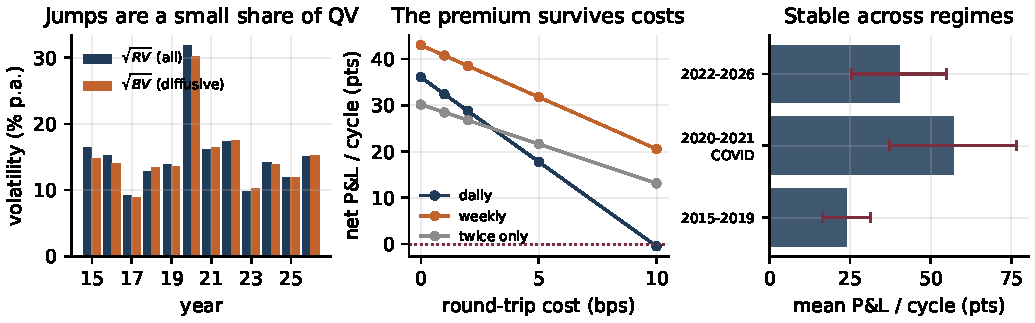
\includegraphics[width=0.98\linewidth]{figures/robustness.pdf}
\end{column}
\begin{column}{0.42\textwidth}
\small
\lead{Jumps.}\ Bipower variation $\tfrac{\pi}{2}\sum|r_i||r_{i-1}|$ is jump-robust. Jump share
$5.60\%$; Barndorff-Nielsen--Shephard $Z=\mathbf{+1.617}$, \textbf{below 1.96}. The no-jump null
is not rejected. About $94\%$ of quadratic variation is diffusive.
\vspace{0.45em}

\lead{Costs.}\ $+32.4$ at 1 bp, $+28.8$ at 2 bps, $+17.8$ at 5 bps. Break-even near
$\mathbf{10}$ bps.
\vspace{0.45em}

\lead{Regimes.}\ 2015--19: $+24.0$ ($t=3.22$). COVID: $+56.9$ ($t=2.91$). 2022--26: $+40.2$
($t=2.74$).
\end{column}
\end{columns}
\vspace{0.2em}
{\scriptsize\color{muted}At zero cost the mean P\&L is \emph{not} a function of rebalance
frequency (spread 22.5 against a typical standard error of 11.9). Frequency buys lower
dispersion, not a higher mean. We claim no optimal frequency.}
\end{frame}

% ---------------- 1973 ----------------
\begin{frame}{``Why use a model from 1973?''}
\begin{inknote}
The model is a \textbf{measurement framework}, not a claim about reality. The P\&L identity
follows from self-financing accounting plus It\^o plus the Black--Scholes PDE, and the
$\sigma_t$ inside it is the \textbf{realised} volatility of whatever path actually occurred.
\end{inknote}
\vspace{0.7em}
\begin{itemize}
  \item We \emph{measured} the three ways the NIFTY breaks the model: clustering, asymmetry,
        fat tails.
  \item The identity still holds at $0.949$ on exactly that data.
  \item That is not luck. The derivation never uses the distributional assumptions.
\end{itemize}
\vspace{0.7em}
\lead{A model can be wrong about the distribution of returns and still be exactly right about
the accounting.}
\end{frame}

% ---------------- methods ----------------
\begin{frame}{Which methods were used}
\begin{columns}[T]
\begin{column}{0.50\textwidth}
\small
\begin{itemize}\itemsep1pt
  \item Exact log-solution of GBM, so zero discretisation error
  \item Monte Carlo, fixed seed, reproducible
  \item Closed-form Black--Scholes price, delta, gamma
  \item Central finite differences, to verify the Greeks only
  \item Trapezoidal quadrature for the It\^o integral
  \item Left-endpoint Riemann sums, as the It\^o convention requires
  \item Ordinary least squares, written out
\end{itemize}
\end{column}
\begin{column}{0.46\textwidth}
\begin{callout}
\small\lead{Not used.}\ No neural network of any kind. No PINNs. No machine learning library.
The repository contains no \texttt{torch}, \texttt{tensorflow}, \texttt{keras} or
\texttt{sklearn}.
\end{callout}
\vspace{0.5em}
\begin{inknote}
\small\lead{On Milstein.}\ In log coordinates $\sigma(t)$ is state-independent, so $b'=0$ and
the correction term vanishes. Milstein reduces to Euler here.
\end{inknote}
\end{column}
\end{columns}
\vspace{0.3em}
{\scriptsize\color{muted}Six modules. Before any result is computed the model layer verifies the
PDE residual to $3.4\times10^{-6}$ relative, the Greeks against finite differences to $10^{-8}$,
and put--call parity to six decimals.}
\end{frame}

% ---------------- real world ----------------
\begin{frame}{Where this is used}
\begin{itemize}\itemsep3pt
  \item \lead{Variance swaps} are priced directly off this identity. The payoff is realised
        variance against a strike.
  \item \lead{The VIX itself} is a variance-swap calculation, which is why India VIX is the
        right quantity to regress against.
  \item \lead{Options market-making.} A gamma book's daily P\&L is explained by exactly this
        decomposition.
  \item \lead{Dispersion trading} and volatility-targeting funds harvest the same premium.
  \item \lead{Carr and Wu (2009)} document the variance risk premium across markets. Our
        $+2.50$ points on the NIFTY is consistent with their findings.
\end{itemize}
\end{frame}

% ---------------- weaknesses ----------------
\begin{frame}{What is genuinely weak}
\begin{enumerate}\itemsep3pt
  \item \lead{The option premium is reconstructed, not quoted.} Both inputs are real market
        data, but the option sold is Black--Scholes evaluated at $\si$ rather than a quote from
        the chain. Verification, measurement and the forecast test are unaffected. What
        inherits the model is the \emph{level} of the backtest P\&L.
  \item \lead{Costs are modelled, not measured.} No market impact, no margin funding.
  \item \lead{Daily closes only.} Intraday data would sharpen both the estimator and the jump
        test, whose asymptotics are weak at $n\approx250$.
  \item \lead{One index, at-the-money calls, flat $r$.} The skew appears in the leverage effect
        but is never priced.
\end{enumerate}
\vspace{0.5em}
The natural next version is a replication on the NSE option chain with its bid--ask spread.
\end{frame}

% ---------------- conclusion ----------------
\begin{frame}{What the project establishes}
In the It\^o framework volatility is a quadratic variation, and that is not a formality.
\vspace{0.7em}
\begin{enumerate}\itemsep4pt
  \item It makes volatility \textbf{measurable} from a single path.
  \item The estimator has a \textbf{verifiable rate and constant}, confirmed to within $2.1\%$
        over a $128\times$ range.
  \item It supplies a \textbf{pathwise identity} converting a forecast error into a P\&L,
        recovered at $0.949$ on real data that violates the model's own assumptions.
\end{enumerate}
\vfill
{\color{accent}\rule{2.0em}{1.4pt}}\par\vspace{0.3em}
{\sffamily\large\color{ink}Thank you. Questions?}
\end{frame}

\end{document}
